\documentclass{exam}
\date{30 Febbraio 2017}
\usepackage[italian]{babel}
\usepackage[T1]{fontenc}
\usepackage{graphicx}
\title{Pendolo quadrifilare}
\author{Francesco Sacco, Francesco Tarantelli, Giovanni Sucameli}
\usepackage{amsmath}
\usepackage{mathtools}
\usepackage{booktabs}
\author{Francesco Tarantelli, Francesco Sacco, Giovanni Sucamelo}
\title{Oscillazioni accoppiate}

\begin{document}
	\maketitle
	\section{Scopo dell'esperienza}
		lo scopo di questa esperienza \'e lo studi del moto di due pendoli accoppiati e, in particolare, del fenomeno dei battimenti


	\section{Cenni Teorici}
		\subsection{Pendolo singolo}
			In questa prima parte si cerca di verificare semplicemente che la pulsazione angolare $\omega_o$ del pendolo fisico senza attrito sia uguale a 
			\begin{equation}
				\omega_o=\sqrt{\frac{mgl}{I}}
			\end{equation}
			In seguito con lo smorzatore si \'e stimato il decadimento $\tau $ dell'ampiezza si oscillazione
			\begin{equation}
				\theta_o(t)=\theta_o(0)e^{-\frac{t}{\tau}}
			\end{equation}
	\subsection{Oscillazioni in fase e in controfase}
		Nelle oscillazioni in fase e in controfase si \'e in sostanza verificato l'equazione del moto dei pendoli nei due modi normali ottenuti dal sistema per un pendolo semplice:

		\begin{equation}
			\begin{cases} 
				m x''_1=-\frac{mg}{l}x_1 + k(x_2-x_1) -\frac{m}{\tau} x'_1 \\
				m x''_2=-\frac{mg}{l}x_2 -  k(x_2-x_1) - \frac{m}{\tau} x'_2
			\end{cases}
		\end{equation}

		che equivale a:

		\begin{equation}
			\begin{bmatrix}
				m & 0 \\
				0 & m
			\end{bmatrix}
			\mathbf{q''}=-
			\begin{bmatrix}
				\frac{mg}{l} + k & -k \\
				-k & \frac{mg}{l} + k \\
			\end{bmatrix}
			\mathbf{q} -
			\begin{bmatrix}
				\frac{m}{\tau} & 0 \\
				0 & \frac{m}{\tau} 
			\end{bmatrix}
			\mathbf{q'} 
		\end{equation}

		dove q=$
		\begin{bmatrix}
			x_1 \\
			x_2
		\end{bmatrix}$
		. La soluzione generale di questa equzione pu\'o essere scritta nella forma:
		\begin{equation}
			\label{eq1}
			x(t)= A_0 e^{-\frac{t}{\tau}}[\cos(\omega_1 t + \phi_1) +\sin(\omega_2 t + \phi_2) ]
		\end{equation}
		in particolare trascurando l'attrito, $\omega_1$ e $\omega_2$ sono uguali alle pulsioni angolari dei modi normali\\($\omega_{fase}^2=\frac{g}{l} \omega_{contro}^2=\frac{g}{l}+2\frac{k}{m} $). L'equazione \ref{eq1} \'e molto importante perch\'e viene utilizzata per descrivere i battimenti.

	\section{Apparato sperimentale}
		\begin{itemize}
			\item Due pendoli
			\item Molla
			\item Due smorzatori
			\item Sistema di acquisizione
		\end{itemize}

	\section{Analisi dati}
		%Smorzato -------------------------------------------------------------------------
		\subsection{Pendolo smorzato}
			Per prima misurazione abbiamo analizzato il moto di un pendolo con galleggiant	e per trovare la costante di smorzamento $\tau$ \\
			\begin{minipage}{0.5\textwidth}
				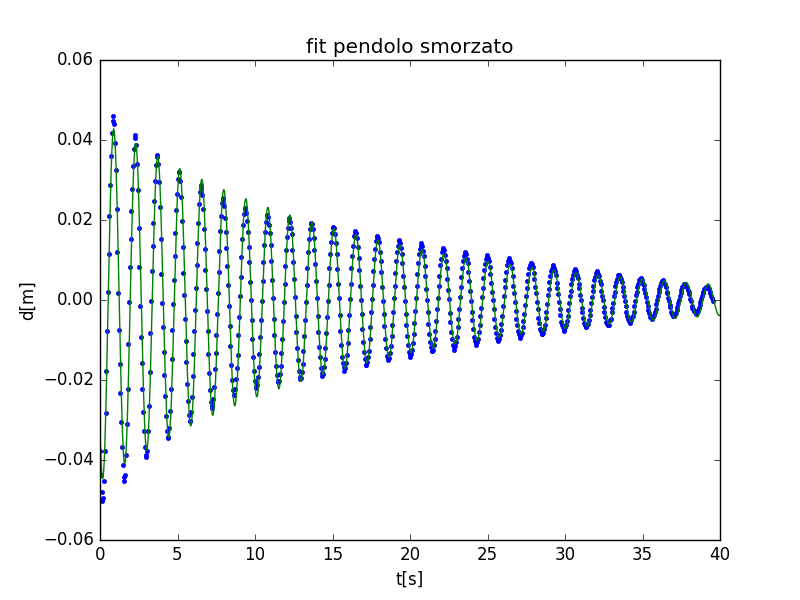
\includegraphics[width=\textwidth]{fit_smorzato}
				\end{minipage}
			\begin{minipage}{0.5\textwidth}
				\begin{tabular}{ll}
					\toprule
					Dati & Parametri ottimali \\
					\midrule
					$\tau$ & $16,24 \pm 0,02$ \\
					$A_{0}$ & $4,51 \pm 6,01(10^{-6})$cm\\
					$\omega$ & $4,42 \pm 2,7(10^{-7})\textrm{s}^{-1}$\\			
					$\phi$ & $3,94 \pm 3,16$\\
					\bottomrule

				\end{tabular}
			\end{minipage}
			Si osservi che i punti sperimentali non seguono perfettamente una curva esponenziale, poich\'e il modello teorico non tiene in considerazione distubi esterni come l'attrito del perno e rumore esterno, e a causa di ci\'o il chi quadro risulta enorme, tuttavia la precisione sull'ampiezza e sul periodo \'e comunque parecchio elevata

		%In fase ---------------------------------------------------------------------------
			\subsection{Pendoli in fase}
			In seguito abbiamo raccolto i dati degli oscillatori in fase, come si pu\'o notare $\omega$ che $\tau$ sono praticamente uguali a quelli dell'oscillatore singolo, questo perch\'e la molla resta alla sua posizione di riposo e quindi \'e come se non ci fosse\\
			\begin{minipage}{0.5\textwidth}
				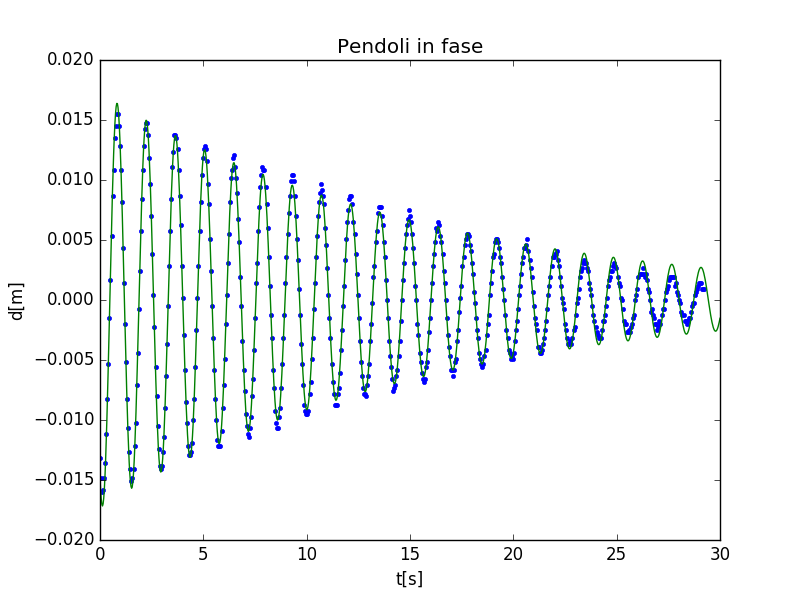
\includegraphics[width=\textwidth]{fase}
			\end{minipage}
			\begin{minipage}{0.5\textwidth}
				\begin{tabular}{ll}
					\toprule
					Dati & Parametri ottimali \\
					\midrule
					$\tau$ & $15,72 \pm 0,02$ \\
					$A_{0}$ & $17,29 \pm 6,75(10^{-7})$cm\\
					$\omega$ & $4,17 \pm 2,41(10^{-5})\textrm{s}^{-1}$\\			
					$\phi$ & $4,45 \pm 2,63(10^{-7})$\\
					\bottomrule
				\end{tabular}
			\end{minipage}
			In questo grafico abbiamo traslato il centro dell'oscillazione a 0, perch\'e la molla spostava la posizione d'equilibrio verso l'altro pendolo, inoltre abbiamo messo solo il grafico di uno dei due pendoli, visto che inserire l'altro risultava ridondante

		%In controfase ---------------------------------------------------------------------
		\subsection{Pendoli in controfase}
			Prima di effettuare la misura dei battimenti abbiamo fatto quella dei pendoli in controfase cosicch\'e ottiniamo i valori di $\omega$ per verificare che ci\'o che \'e scritto nei cenni teorici\\
			\begin{minipage}{0.5\textwidth}
				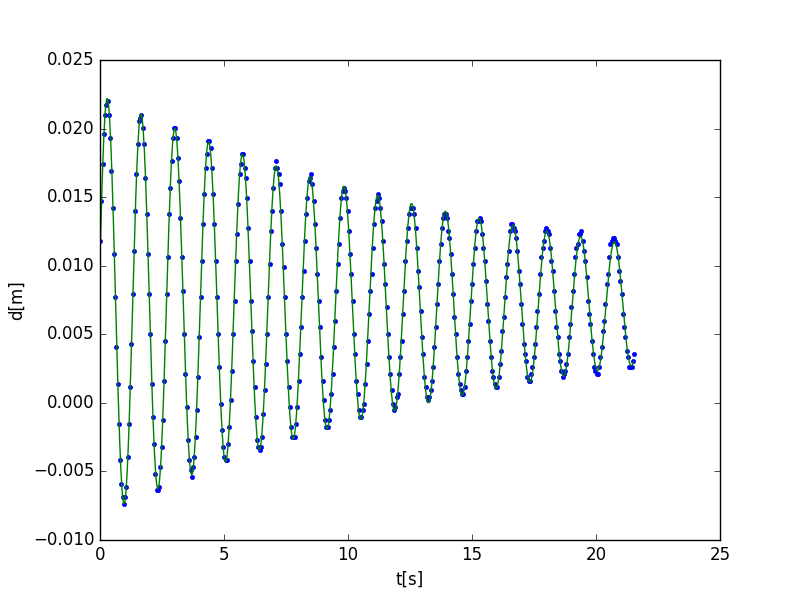
\includegraphics[width=\textwidth]{controfase}
				\end{minipage}
			\begin{minipage}{0.5\textwidth}
				\begin{tabular}{ll}
					\toprule
					Dati & Parametri ottimali \\
					\midrule
					$\tau$ & $17,27 \pm 0,03$ \\
					$A_{0}$ & $1,53 \pm 4,89(10^{-7})$cm\\
					$\omega$ & $6,51 \pm 2,11(10^{-5})\textrm{s}^{-1}$\\			
					$\phi$ & $4,61 \pm 2,87(10^{-7})$\\
					\bottomrule
				\end{tabular}
			\end{minipage}
			La prima cosa che salta all'occhio \'e che $\omega$ è aumentato come si ci aspettava, mentr $\tau$ non cambia di molto \'e
		%Battimenti ------------------------------------------------------------------------
		\subsection {Battimenti}
			Dulcis in fundu, abbiamo fatto la raccolta dati dei battimenti e fatto il fit. Questo fit è risultato parecchio impegnativo perch\'e sembrava non voler trovare il minimo $\chi^2$, ma alla fine cel'abbiamo fatta.\\
			\begin{minipage}{0.5\textwidth}
				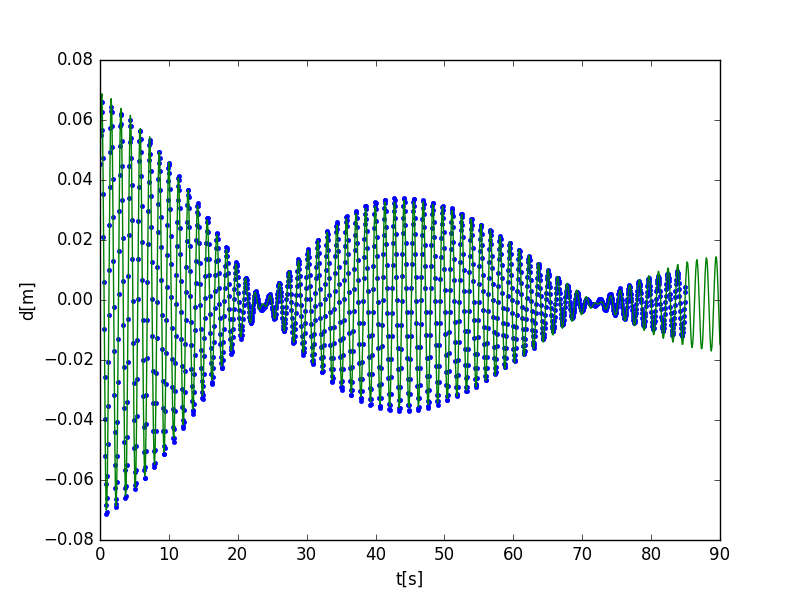
\includegraphics[width=\textwidth]{Battimenti}
				\end{minipage}
			\begin{minipage}{0.5\textwidth}
				\begin{tabular}{ll}
					\toprule
					Dati & Parametri ottimali \\
					\midrule
					$\tau$ & $17,27 \pm 0,03$ \\
					$A_{0}$ & $1,53 \pm 4,89(10^{-7})$cm\\
					$\omega_{a}$ & $6,51 \pm 2,11(10^{-5})\textrm{s}^{-1}$\\
					$\omega_{b}$ & $6,51 \pm 2,11(10^{-5})\textrm{s}^{-1}$\\			
					$\phi$ & $4,61 \pm 2,87(10^{-7})$\\
					\bottomrule
				\end{tabular}
			\end{minipage}

\end{document}